\section{ZLP parametrisation from vacuum spectra}
\label{sec:results_vacuum}

We now move to discuss the application of the strategy presented in the previous
section to the parametrisation of ZLP spectra acquired in vacuum.
%
Applying our model to this case has a two-fold motivation.
%
First of all, we aim to demonstrate that the model is sufficiently flexible
to effectively reproduce the
input EELS measurements for a range of variations of the operation parameters of the microscope.
%
Second, it allows one to provide a calibrated prediction
useful for the case of the in-sample measurements.
%
Such calibration is necessary since, as explained in Sect.~\ref{sec:training}, some of the model
hyper-parameters are determined by comparing intensity shape profiles
between spectra taken in vacuum and in sample.

In this section, first of all we present the input dataset and motivate the choice
of training settings and model hyperparameters.
%
Then we validate the model training by assessing the fit quality.
%
Lastly, we study the dependence of the model output in its various input
variables, extrapolate  its predictions to new operation
conditions, and study the dependence of the model uncertainties upon
restricting the training dataset.

\subsection{Training settings}

In Table~\ref{table:vacuumdata} we collect the main properties of the EELS spectra
acquired in vacuum to train the neural
network model.  For each set of spectra, we indicate the exposure time $t_{\rm exp}$, the beam energy
$E_b$, the number of spectra $N_{\rm sp}$ recorded for these operation conditions, the number $n_{\rm dat}$ of
bins in each spectrum, the range in electron energy loss $\Delta E$,
and the average full width at half maximum (FWHM)
evaluated over the $N_{\rm sp}$ spectra with the corresponding standard deviation.
%
The spectra  listed on Table~\ref{table:vacuumdata}
were acquired with a ARM200F Mono-JEOL microscope equipped
with a GIF continuum spectrometer, see also Methods.
%
We point out that since here
we are interested in the low-loss region, $\Delta E_{\rm max}$ does not need
to be too large, and anyway the $\Delta E\to \infty$ behaviour of the model is fixed
by the constraint implemented by Eq.~(\ref{eq:chi2modified}).

%%%%%%%%%%%%%%%%%%%%%%%%%%%%%%%%%%%%%%%%%%%%%%%%%%%%%%%%%%%%%%%%%%%%%%%%%%%%%%%%%%%%%%%%%%%%%
%%%%%%%%%%%%%%%%%%%%%%%%%%%%%%%%%%%%%%%%%%%%%%%%%%%%%%%%%%%%%%%%%%%%%%%%%%%%%%%%%%%%%%%%%%%%%
\begin{table}[t]
  \begin{center}
            \renewcommand{\arraystretch}{1.50}
  \begin{tabular}{@{}ccccccccc}
\br
Set & $t_{\rm exp}$ {(}ms{)} & $E_{\rm b}$ {(}keV{)} & $N_{\rm sp}$ & $n_{\rm dat}$ & $\Delta E_{\rm min}$~(eV)  & $\Delta E_{\rm max}$~(eV)  & FWHM~(meV)  \\ 
\mr
1        & 100                 & 200                  & 15          & 2048               & -0.96              & 8.51     & $47\pm7 $         \\
2        & 100                 & 60                   & 7           & 2048               & -0.54              & 5.59    & 
$ 50 \pm 4$         \\
3        & 10                  & 200                  & 6          & 2048               & -0.75              & 5.18      & 
$ 26 \pm 3$         \\
4        & 10                  & 60                   & 6           & 2048               & -0.40              & 4.78       & 
$ 34\pm 2$         \\ 
\br
  \end{tabular}
    \end{center}
  \caption{\small Summary of the main properties of the EELS spectra acquired in vacuum to train the neural
    network model.  For each set of spectra, we indicate the exposure time $t_{\rm exp}$, the beam energy
    $E_b$, the number of spectra $N_{\rm sp}$ recorded for these operation conditions, the number $n_{\rm dat}$ of
    bins in each spectrum, the range in electron energy loss $\Delta E$,
    and the average FWHM evaluated over the $N_{\rm sp}$ spectra with the corresponding standard deviation
  }
   \label{table:vacuumdata}
\end{table}
%%%%%%%%%%%%%%%%%%%%%%%%%%%%%%%%%%%%%%%%%%%%%%%%%%%%%%%%%%%%%%%%%%%%%%%%%%%%%%%%%%%%%%%%%%%%%%%%%5
%%%%%%%%%%%%%%%%%%%%%%%%%%%%%%%%%%%%%%%%%%%%%%%%%%%%%%%%%%%%%%%%%%%%%%%%%%%%%%%%%%%%%%%%%%%%%

The energy resolution of these spectra, quantified by the average value of their FWHM, ranges
from 26 meV to 50 meV depending on the specific operation conditions of the microscope,
with an standard deviation between 2 and 7 meV.
%
The value of the FWHM varies only mildly with the value of the beam energy $E_b$
but grows rapidly for spectra collected with larger exposure times $t_{\rm exp}$.
%
A total of almost $7\times 10^4$ independent measurements will be used for the ZLP model
training on the vacuum spectra.
%
As will be highlighted in Sects.~\ref{eq:depdeltae} and~\ref{eq:depebeam}, one of the advantages of our ZLP model is that it can extrapolate its predictions
to other operation conditions beyond the specific ones used for the training
and listed in Table~\ref{table:vacuumdata}.

Following the strategy presented in Sect.~\ref{sec:methodology}, first of all we combine the $N_{\rm sp}$ spectra
corresponding to each of the four sets of operation conditions and determine the statistical uncertainty
associated to each energy loss bin by means of Eq.~(\ref{eq:sigmaiexp}).
%
For each of the training sets, we need to determine the value
of $\Delta E_{\rm pd}^{\rm (min)}~(=\Delta E_{\rm II})$
that defines the range for which we add the  pseudo-data
that imposes the correct $\Delta E \to \infty$ limit of the model.
%
This value is fixed by the condition that
ratio between the central experimental value of the 
EELS intensity and its corresponding uncertainty,
Eq.~(\ref{eq:pdlocation}), satisfies $\mathcal{R}_{\rm sig}\simeq 1$.
      
%%%%%%%%%%%%%%%%%%%%%%%%%%%%%%%%%%%%%%%%%%%%%%%%%%%%%%%%%%%%%%%%%%%%%%%%%%%%%%%%%%%%%%%%%%%%%%%%%%%%%%%%%%%%
\begin{figure}[t]
  \centering
  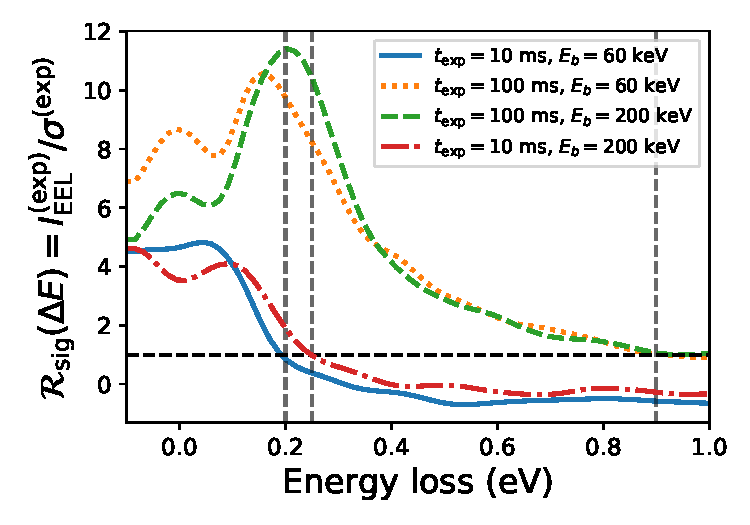
\includegraphics[width=125mm]{plots/intensity_to_error_ratio.pdf}
  \caption{\small The ratio $\mathcal{R}_{\rm sig}(\Delta E)$
    between the central experimental value of the 
    EELS intensity distribution and its corresponding
    uncertainty.
    %
    Results are shown for the four combinations of $t_{\rm exp}$
    and $E_{b}$ listed in Table~\ref{table:vacuumdata}.
    %
    The vertical dashed lines mark the values of $\Delta E$ for which
    $\mathcal{R}_{\rm sig}\simeq 1$, which indicates when the
    data is dominated by statistical noise.
  }
  \label{fig:intensityratio}
\end{figure}
%%%%%%%%%%%%%%%%%%%%%%%%%%%%%%%%%%%%%%%%%%%%%%%%%%%%%%%%%%%%%%%%%%%%%%%%%%%%%%%%%%%%%%%%%%%%%%%%%%%%%%%%%%%%%%%%%

Fig.~\ref{fig:intensityratio} displays this ratio
for the four combinations of $t_{\rm exp}$
and $E_{b}$ listed in Table~\ref{table:vacuumdata}.
%
The vertical dashed lines indicate the values of $\Delta E$ for which
$\mathcal{R}_{\rm sig}$ becomes smaller than unity.
%
For larger $\Delta E$, the EELS spectra become
consistent with zero within uncertainties and can thus be discarded and replaced
by the pseudo-data constraints.
%
The total uncertainty of the pseudo-data points is then chosen to be
\be
\sigma_j^{(\rm pd)} = \frac{1}{10}I_{{\rm EEL}}^{\rm (exp)}\lp \Delta E = \Delta E_{\rm pd}^{\rm (min)}\rp \,, \quad 
j= 1,\ldots,N_{\rm pd} \, .
\ee
The factor of 1/10 is found to be suitable to ensure that the constraint
is enforced without distorting
the training to the experimental data.
%
We observe from Fig.~\ref{fig:intensityratio} that $\Delta E_{\rm pd}^{\rm (min)}$ depends
the operation conditions, with $\Delta E_{\rm pd}^{\rm (min)} \simeq 200$ meV for $t_{\rm exp}=10$ ms
and $\simeq  900$ meV for 100 ms, roughly independent on the value of the beam energy $E_b$.

The input experimental measurements listed in Table~\ref{table:vacuumdata} are used
to generate a sample of $N_{\rm rep}=500$ Monte Carlo replicas
and to train an individual neural network to each of these replicas.
%
The end result of the procedure is a set of model replicas,
\be
\label{eq:modelreplicas}
I_{\rm ZLP}^{\rm (mod)(k)}(\Delta E, E_{b},t_{\rm exp}) \, , \quad k=1,\ldots,N_{\rm rep} \, ,
\ee
which can be used to provide a prediction for the intensity of the ZLP
for arbitrary values of $\Delta E$,  $E_{b}$, and $t_{\rm exp}$.
%
Eq~(\ref{eq:modelreplicas})
provides the sought-for representation of the probability density in the space of ZLP models.
%
By means of this sample of replicas, one can evaluate
statistical estimators such as averages, variances, and correlations (as well
as higher moments) as follows:
\be
\label{eq:average}
\la I_{\rm ZLP}^{\rm (mod)}( \{z_1\}) \ra = \frac{1}{N_{\rm rep}}\sum_{k=1}^{N_{\rm rep}}
I_{\rm ZLP}^{\rm (mod)(k)}( \{z_1\}) \, ,
\ee
\be
\label{eq:standarddev}
\sigma_{I_{\rm ZLP}}^{\rm (mod)}( \{z_1\})  = \lp \frac{1}{N_{\rm rep}-1} \sum_{k=1}^{N_{\rm rep}}
\lp  I_{\rm ZLP}^{\rm (mod)(k)}  - \la I_{\rm ZLP}^{\rm (mod)}  \ra   \rp \rp^{1/2} \, ,
\ee
\be
\rho \lp \{z_1\},\{z_2\}\rp = \frac{ \la I_{\rm ZLP}^{\rm (mod)}( \{z_1\} ) I_{\rm ZLP}^{\rm (mod)}( \{z_2\} ) \ra
- \la I_{\rm ZLP}^{\rm (mod)}( \{z_1\} )\ra \la I_{\rm ZLP}^{\rm (mod)}( \{z_2\} ) \ra}{\sigma_{I_{\rm ZLP}}^{\rm (mod)}( \{z_1\} )\sigma_{I_{\rm ZLP}}^{\rm (mod)}( \{z_2\} )} \, ,
\ee
where as in the previous section $\{z_l\}$ denotes a possible set of input variables for the model,
here $\{z_l\}=\lp \Delta E_l, E_{b,l},t_{{\rm exp},l}\rp$.

\subsection{Fit quality}

We would like now to evaluate the overall fit quality of the neural network
model and demonstrate that it is flexible enough
to describe the available input datasets.
%
In Table~\ref{table:chi2summary} we indicate the values of the final $\chi^2$ per data point,
Eq.~(\ref{eq:chi2_final}), as well as the average values of the cost
function Eq.~(\ref{eq:chi2}) evaluated
over the training and validation subsets, for each of the four sets of spectra listed in
Table~\ref{table:vacuumdata} as well as for the total dataset.
%
We recall that for a satisfactory training one expects $\chi^2 \simeq 1$
and $\la E_{\rm tr}\ra \simeq \la E_{\rm val}\ra \simeq 2 $~\cite{Forte:2002fg}.
%
From the results of this table we find that, while our values
are  consistent with a reasonably good training,
somewhat lower values than expected are obtained,
for instance $\chi^2_{\rm tot}\simeq 0.8$ for the total dataset.
%
This suggests that correlations between the input data points might be partially missing, since neglecting
them often results into a moderate overestimate of the experimental uncertainties.

%%%%%%%%%%%%%%%%%%%%%%%%%%%%%%%%%%%%%%%%%%%%%%%%%%%%%%%%%%%%%%%%%%%%%%%%%%%%%%%%%%%%%%%%%%%%%
%%%%%%%%%%%%%%%%%%%%%%%%%%%%%%%%%%%%%%%%%%%%%%%%%%%%%%%%%%%%%%%%%%%%%%%%%%%%%%%%%%%%%%%%%%%%%
\begin{table}[t]
  \begin{center}
            \renewcommand{\arraystretch}{1.35}
  \begin{tabular}{@{}cccc}
\br
$\quad$Set$\quad$ & $\qquad \chi^2\qquad$  &  $\qquad\la E_{\rm tr}\ra\qquad$   &  $\qquad\la E_{\rm val}\ra\qquad$ \\
\mr
1        &           1.00        &      1.70            &  1.97  \\
2        &           0.73        &     1.41            &  1.77  \\
3        &           0.70        &    1.39            &  1.80  \\
4        &           0.60        &    1.20            &  1.76  \\
\mr
Total    &           0.77        &    1.47           &  1.85  \\
\br
  \end{tabular}
    \end{center}
  \caption{\small \small The values of the $\chi^2$ per data point,
    Eq.~(\ref{eq:chi2_final}), as well as the average values of the cost function Eq.~(\ref{eq:chi2})
    over the training $\la E_{\rm tr}\ra$ and validation $\la E_{\rm val}\ra$ subsets, for each of the four sets of spectra listed in
    Table~\ref{table:vacuumdata} as well as for the total dataset used in the present analysis.
  }
   \label{table:chi2summary}
\end{table}
%%%%%%%%%%%%%%%%%%%%%%%%%%%%%%%%%%%%%%%%%%%%%%%%%%%%%%%%%%%%%%%%%%%%%%%%%%%%%%%%%%%%%%%%%%%%%%%%%5
%%%%%%%%%%%%%%%%%%%%%%%%%%%%%%%%%%%%%%%%%%%%%%%%%%%%%%%%%%%%%%%%%%%%%%%%%%%%%%%%%%%%%%%%%%%%%

Then Fig.~\ref{fig:chi2_distributions} displays separately the $\chi^2$  distributions
evaluated for the training and validation sets
of the $N_{\rm rep}=500$ replicas of the sample trained on the spectra
listed in Table~\ref{table:vacuumdata}.
%
Note that the training/validation partition differs at random for each replica.
%
The $\chi^2_{\rm tr}$ distribution peaks at $\chi^2_{\rm tr}\simeq 0.7$,
indicating that a satisfactory model training
has been achieved, but also that the errors on the input data points might have
been slightly overestimated.
%
We emphasize that the stopping criterion for the neural net training adopted here never considers
the absolute values of the error function and determines proper learning entirely from
the global minima of $E_{\rm val}^{(k)}$.
%
From Fig.~\ref{fig:chi2_distributions} we also observe that  the validation
distribution peaks at
a slighter higher value, $\chi^2_{\rm val}\simeq 1$, and
is broader that its corresponding training counterpart.
%
These results confirm both that a satisfactory model training that prevents overlearning
has been achieved as well as an appropriate estimate of the statistical uncertainties
associated to the original EEL spectra.

%%%%%%%%%%%%%%%%%%%%%%%%%%%%%%%%%%%%%%%%%%%%%%%%%%%%%%%%%%%%%%%%%%%%%%%%%%%%%%%%%%%%%%%%%%%%%%%%%%%%%%%%%%%%
\begin{figure}[t]
    \centering
    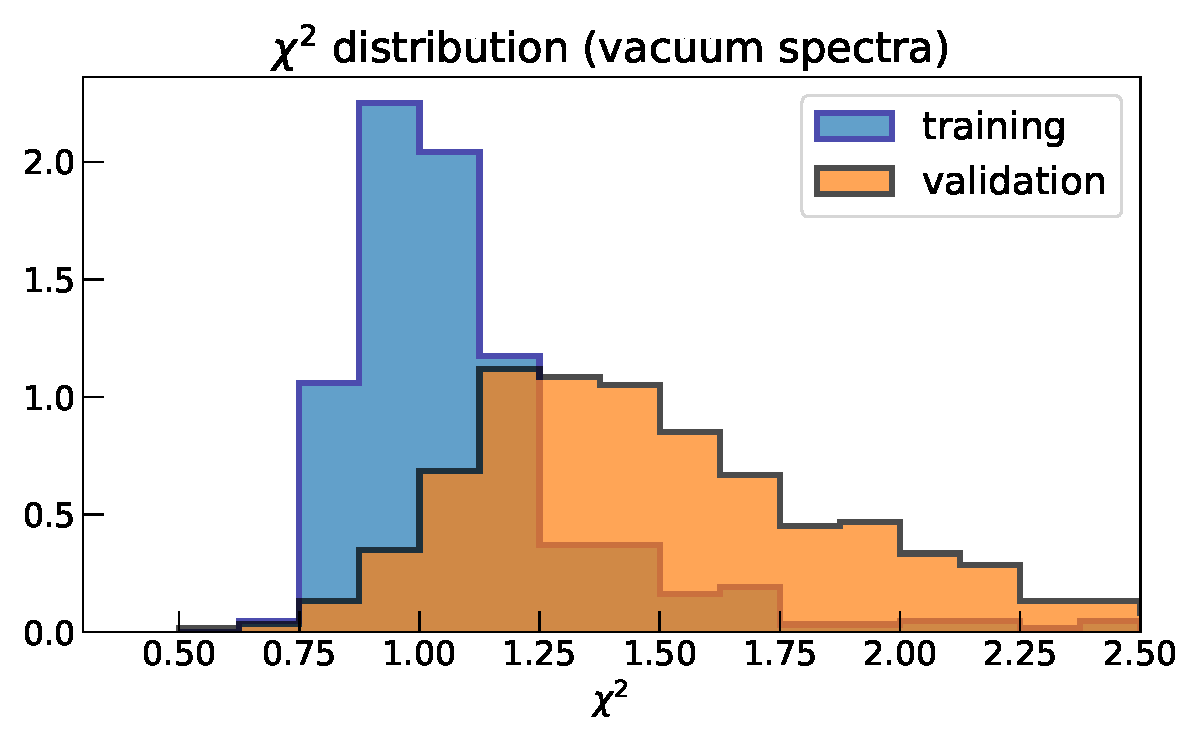
\includegraphics[width=120mm]{plots/chi2_distributions.pdf}
    \caption{\small The distribution of the $\chi^2$ per data point evaluated
      separately for the training and validation sets over
      the $N_{\rm rep}=500$ replicas trained on the spectra
      listed in Table~\ref{table:vacuumdata}.}
    \label{fig:chi2_distributions}
\end{figure}
%%%%%%%%%%%%%%%%%%%%%%%%%%%%%%%%%%%%%%%%%%%%%%%%%%%%%%%%%%%%%%%%%%%%%%%%%%%%%%%%%%%%%%%%%%%%%%%%%%%%%%%%%%%%%%%%%%%

\subsection{Dependence on the electron energy loss}
\label{eq:depdeltae}

Having demonstrated that our neural network model provides a satisfactory description
of the input EEL spectra, we now present its  predictions for specific
choices of the input parameters.
%
First of all, we investigate the dependence of the results as a function of the
electron energy loss.
%
Fig.~\ref{fig:EELS_vacuum_DeltaE} displays the central value and 68\% confidence level uncertainty band
for the ZLP model as a function
of electron energy loss $\Delta E$
evaluated using Eqns.~(\ref{eq:average}) and~(\ref{eq:standarddev}).
%
We display results corresponding to 
three different values of $E_b$  and for both
$t_{\rm exp}=10$ ms and  $100$ ms.
%
We emphasize that no measurements with $E_b=120$ keV have been used in the training and thus our prediction
in that case arises purely from the model interpolation.
%
It is interesting to note how both the overall normalisation and the shape of
the predicted ZLP depend on the specific operating conditions.

%%%%%%%%%%%%%%%%%%%%%%%%%%%%%%%%%%%%%%%%%%%%%%%%%%%%%%%%%%%%%%%%%%%%%%%%%%%%%%%%%%%%%%%
\begin{figure}[t]
    \centering
    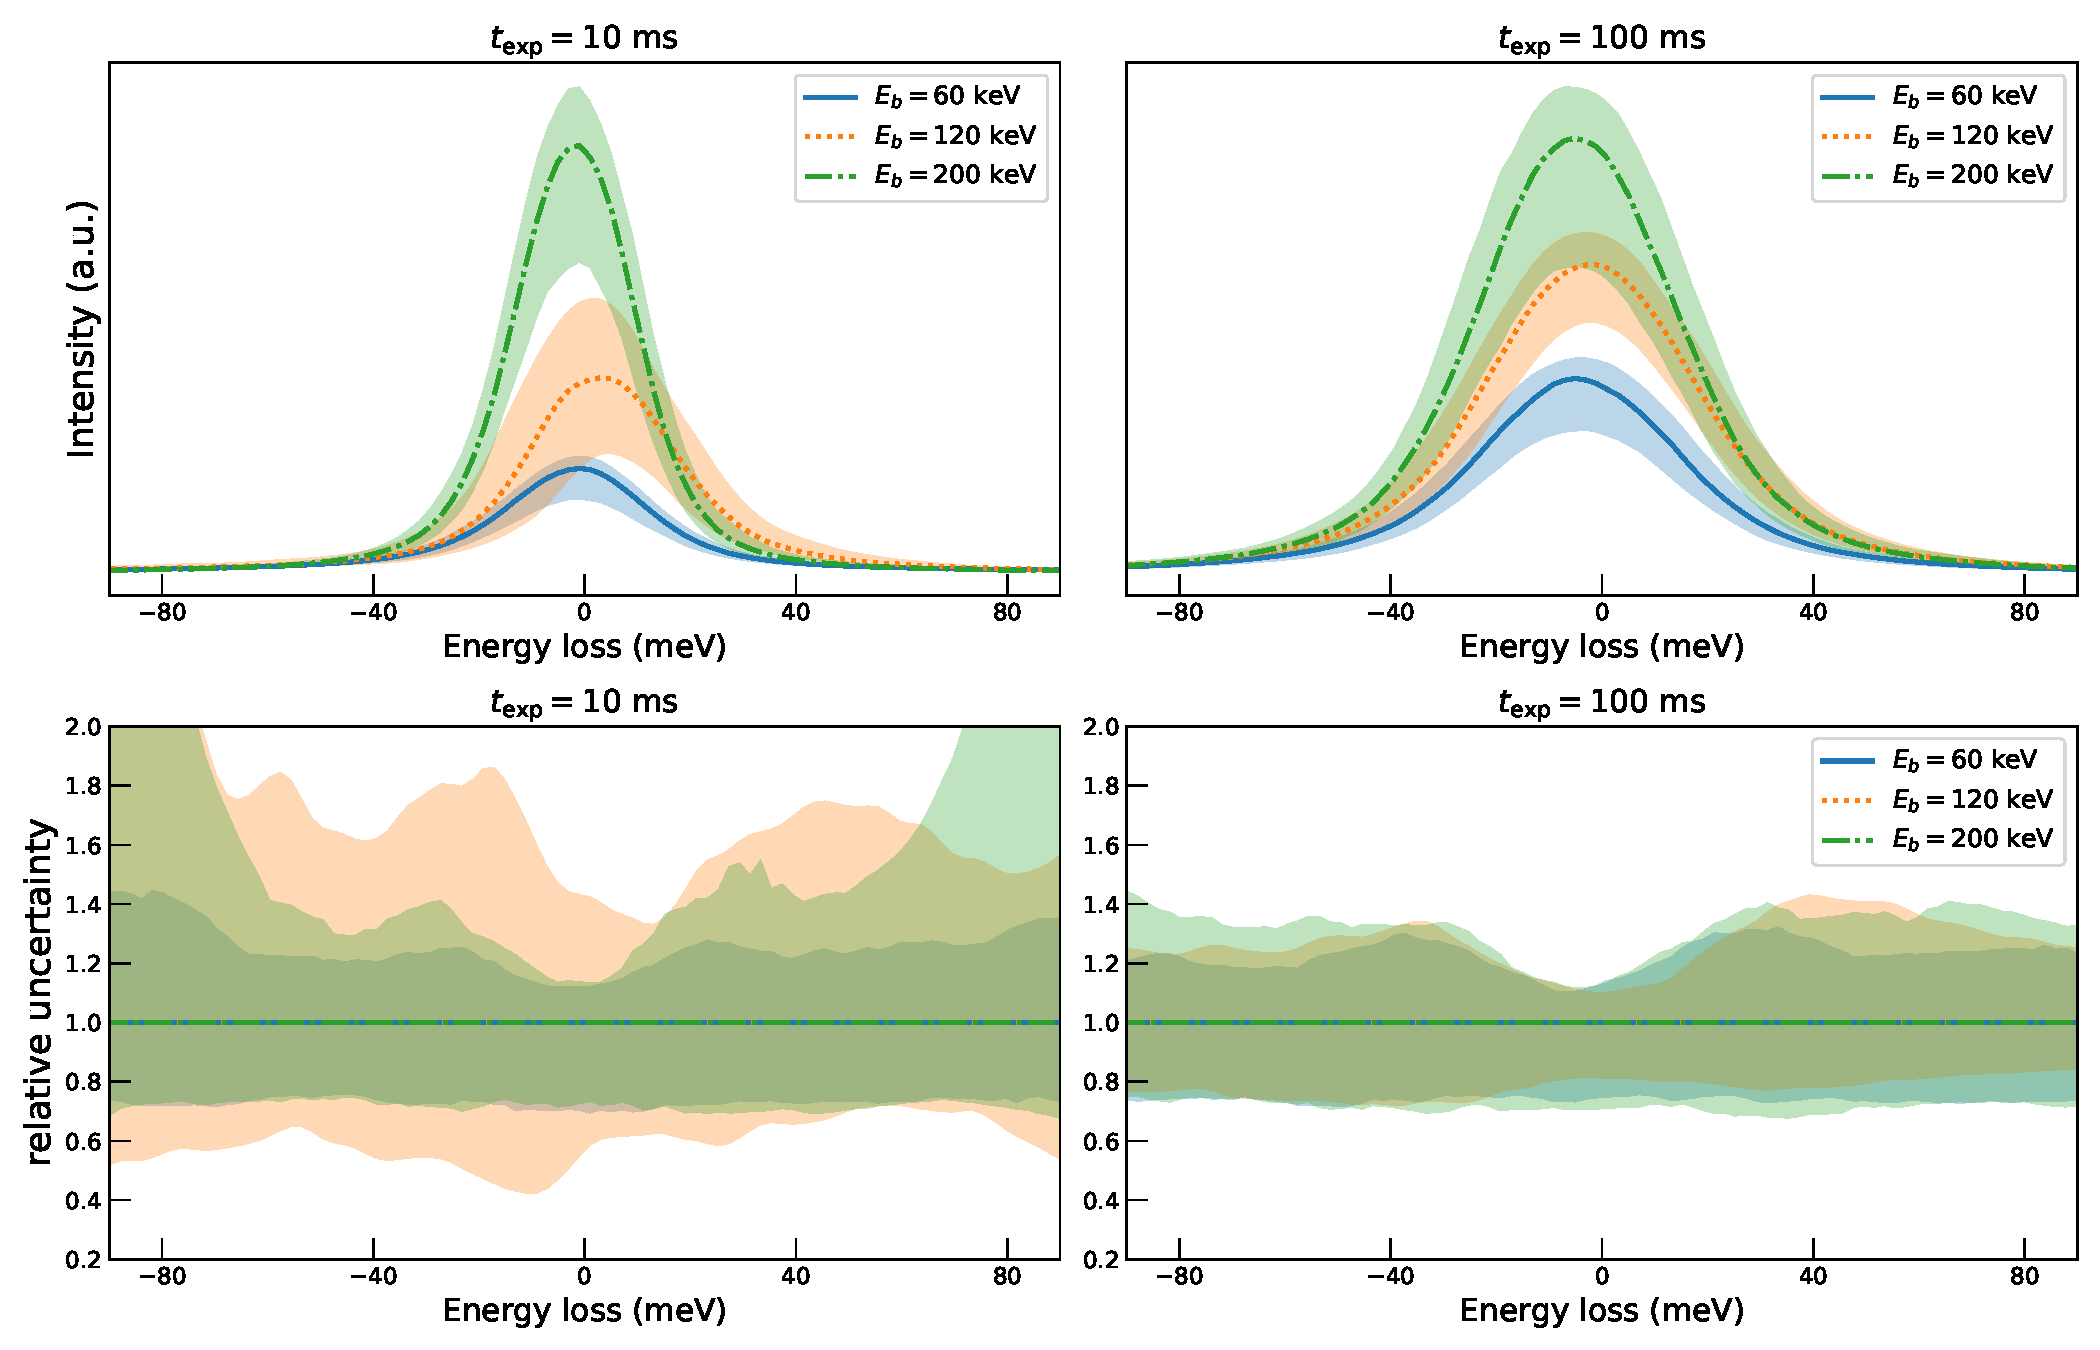
\includegraphics[width=170mm]{plots/deltaE_dependence_vacuum.pdf}
    \caption{\small Top: the central value and 68\% confidence level uncertainty band
      for the ZLP model as a function
      of electron energy loss $\Delta E$
      evaluated using Eqns.~(\ref{eq:average}) and~(\ref{eq:standarddev}).
      %
      We display results corresponding to 
      three different values of $E_b$  and for both
      $t_{\rm exp}=10$ ms (left)  and $t_{\rm exp}=100$ ms (right panel).
      %
      Note that no training data with $E_b=120$ keV has been used and thus our prediction
      in that case arises purely from the model interpolation.
      %
      Bottom: the corresponding relative uncertainty as a function of $\Delta E$
      for each of the three values of $E_b$.
      \label{fig:EELS_vacuum_DeltaE}}
\end{figure}
%%%%%%%%%%%%%%%%%%%%%%%%%%%%%%%%%%%%%%%%%%%%%%%%%%%%%%%%%%%%%%%%%%%%%%%%%%%%%%%%%%%%%%%%%


In the bottom panels of Fig.~\ref{fig:EELS_vacuum_DeltaE} we show
the corresponding relative uncertainties as a function of $\Delta E$
for each of the three values of $E_b$.
%
Recall that in this work we allow for non-Gaussian distributions and thus the central
value is the median of the distribution and the error band in general will
be asymmetric.
%
In the case of the $t_{\rm exp}=10$ ms results, we see how the model prediction
at $E_b=120$ keV typically exhibits larger uncertainties than the predictions
for the two values of $E_b$ for which we have training data.
%
In the case of $t_{\rm exp}=100$ ms instead, the model predictions display very similar
uncertainties for the three values of $E_b$, which furthermore depend only mildly on $\Delta E$.
%
One finds there that the uncertainties associated to the ZLP model are $\simeq 20\%$
for $|\Delta E| \lsim 100~{\rm meV}$.



For the purpose of the second part of this work, it is important
to assess how the model results are modified once a subset of the data points
are excluded from the fit.
%
As illustrated in Fig.~\ref{fig:EELS_toy}, when training the model on sample spectra, the
region defined by
with $\Delta E_{\rm I} \le \Delta E \le \Delta E_{\rm II}$ will be removed from the training dataset to avoid the
contamination from the inelastic contributions.
%
To emulate the effects of such cut, 
Fig.~\ref{fig:EELS_vacuum_DeltaE_unc} displays
the relative uncertainty in the model predictions for $I_{\rm ZLP}(\Delta E)$
as a function of the energy loss for $E_b=200$ keV and $t_{\rm exp}=10$ ms 
and 100 ms.
%
We show results for three different cases: first of all, one without any cut
in the training dataset, and then for two cases where data points with $\Delta E \ge \Delta E_{\rm cut}$
are removed from the training dataset.
%
We consider two values of $\Delta E_{\rm cut}$, namely 50 meV and 100 meV, indicated
with vertical dash-dotted lines.
%
In both cases, data points are removed up until $\Delta E =$ 800 meV. The pseudo-data points 
that enforce the $I_{\rm EEL}(\Delta E)\to 0$ condition are present
in all three cases in the region 800 meV $\le \Delta E \le 1~{\rm eV}$. 

%%%%%%%%%%%%%%%%%%%%%%%%%%%%%%%%%%%%%%%%%%%%%%%%%%%%%%%%%%%%%%%%%%%%%%%%%%%%%%
\begin{figure}[t]
    \centering
    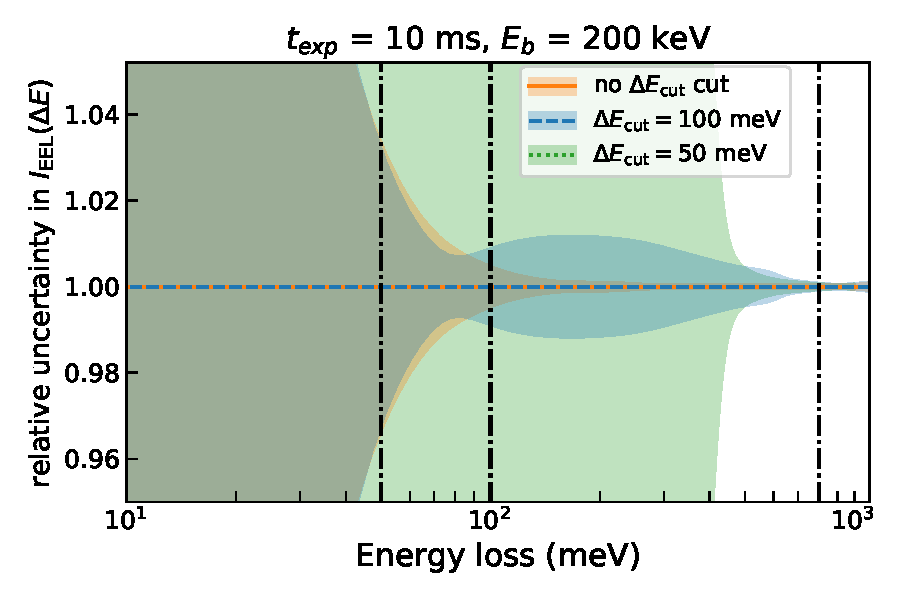
\includegraphics[width=0.49\textwidth]{plots/prediction_with_cut_10ms.pdf}
    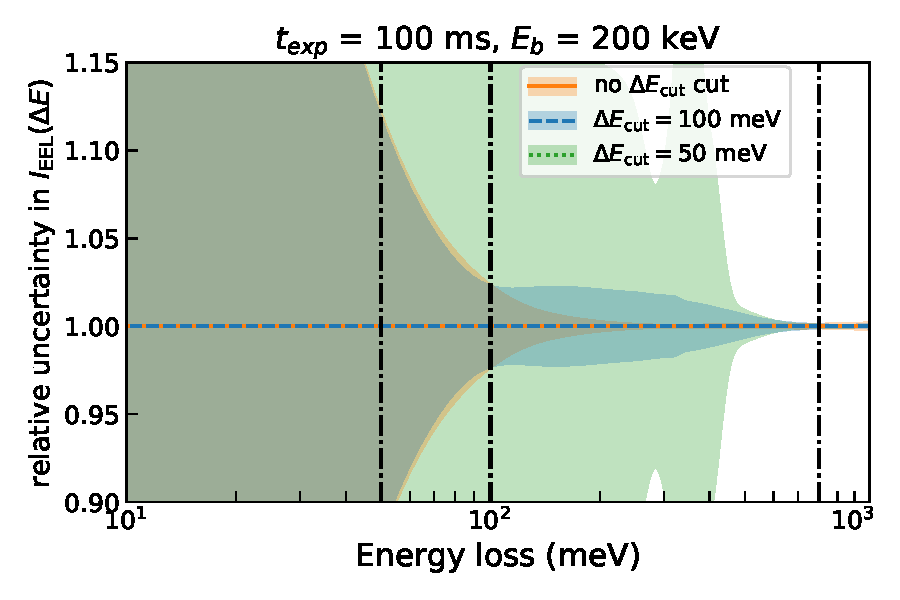
\includegraphics[width=0.49\textwidth]{plots/prediction_with_cut_100ms.pdf}
    \caption{\small The relative uncertainty in the model predictions for $I_{\rm EEL}(\Delta E)$
      as a function of the energy loss for $E_b=200$ keV and $t_{\rm exp}=10$ ms (left)
      and 100 ms (right panel).
      %
      We show results for three different cases: without any cut
      in the training dataset, and where the data points with $\Delta E \ge \Delta E_{\rm cut}$
      are removed from the training dataset for two different values
      of $\Delta E_{\rm cut}$.
      %
      The same pseudo-data points that enforce $I_{\rm EEL}(\Delta E)\to 0$ are present
      in all three cases.
      \label{fig:EELS_vacuum_DeltaE_unc}}
\end{figure}
%%%%%%%%%%%%%%%%%%%%%%%%%%%%%%%%%%%%%%%%%%%%%%%%%%%%%%%%%%%%%%%%%%%%%%%%%%%%%%%%


From this comparison one can observe how the model predictions become markedly more uncertain
once a subset of the training data is cut away, as expected due to the effect of the information
loss.
%
While for the cut $\Delta E_{\rm cut}=100$ meV the increase in model uncertainty is only moderate
as compared with the baseline fit where no cut is performed (since for this value of $\Delta E$
uncertainties are small to begin with), rather more dramatic effects are observed
for a value of the cut $\Delta E_{\rm cut}=50$ meV.
%
This comparison highlights how ideally we would like to keep as many data points
in the training set for the ZLP model, provided of course one can verify that the
possible contributions to the spectra related to inelastic scatterings from the
sample can be neglected.

\subsection{Dependence on beam energy and exposure time }
\label{eq:depebeam}

As indicated in Table~\ref{table:vacuumdata}, the training dataset contains
spectra taken at two values of the electron beam energy, $E_b=60$ keV and 200 keV.
%
The left panel of Fig.~\ref{fig:extrapolbeam} displays the predictions for the FWHM of the zero loss peak
(and its corresponding uncertainty) as a function of the beam energy $E_b$
for two values of the exposure time, $t_{\rm exp}=10$ ms and 100 ms.
%
The vertical dashed lines indicate the two values of $E_b$ for which spectra
are part of the training dataset.
%
This comparison illustrates how the model uncertainty differs between the data region
(near $E_b=60$ keV and 200 keV), the interpolation region (for $E_b$ between 60 and 200 keV),
and the extrapolation regions (for $E_b$ below 60 keV and above 200 keV).
%
In the case of $t_{\rm exp}=100$ ms for example, we observe that the model interpolates reasonably well
between the measured values of $E_b$ and that uncertainties increase
markedly in the extrapolation region above $E_b=200$ keV.
      
%%%%%%%%%%%%%%%%%%%%%%%%%%%%%%%%%%%%%%%%%%%%%%%%%%%%%%%%%%%%%%%%%%%%%%%%%%%%%%%%%%%%%%%
\begin{figure}[t]
    \centering
    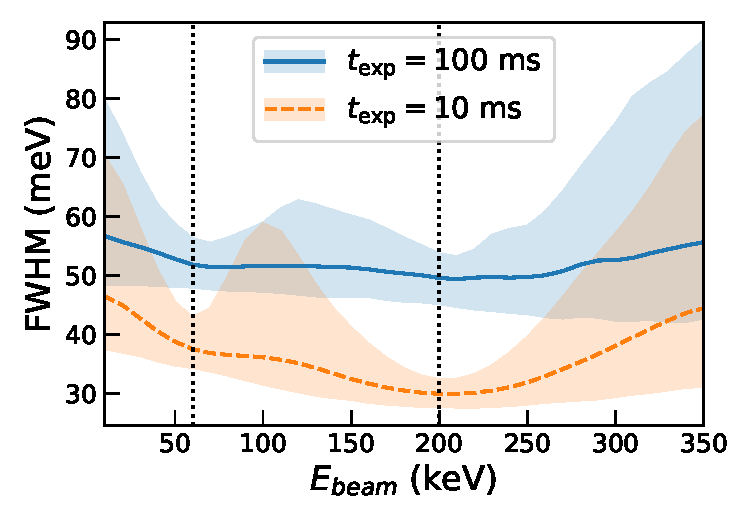
\includegraphics[width=0.49\textwidth]{plots/Ebeam_extrapolation.pdf}
    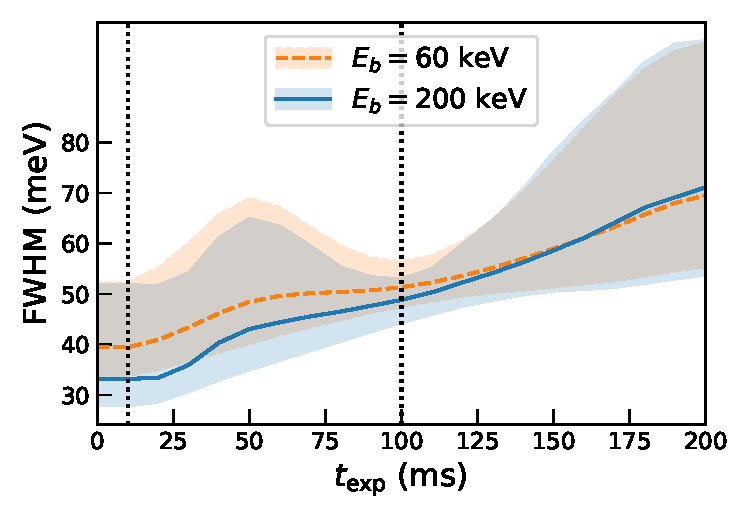
\includegraphics[width=0.49\textwidth]{plots/time_extrapolation.pdf}
    \caption{\small The model predictions for the FWHM of the zero loss peak
      with its corresponding uncertainty as a function of the beam energy $E_b$
      for two values of the exposure time (left panel)
      and as a function of $t_{\rm exp}$ for two values of $E_b$ (right panel).
      %
      The vertical dashed lines indicate the values of the
      corresponding microscope operation parameter for which we have training data.
    }
    \label{fig:extrapolbeam}
\end{figure}
%%%%%%%%%%%%%%%%%%%%%%%%%%%%%%%%%%%%%%%%%%%%%%%%%%%%%%%%%%%%%%%%%%%%%%%%%%%%%%%%%%%%%%%%%%%%

From this comparison one can also observe how as expected the uncertainty in the  prediction for
the FWHM of the ZLP is the smallest close to the values of $E_b$ for which one has training data.
%
The uncertainties increase but only in a moderate way in the interpolation region, indicating that
the model can be applied to reliably predict the features of the ZLP for other values of the electron
energy beam (assuming that all other operation conditions of the microscope are unchanged).
%
The errors then increase rapidly in the extrapolation region, which is a characteristic
(and desirable) feature of  neural network models.
%
Indeed, as soon as the model departs from the data region there exists a very large
number of different functional form models for $I_{\rm ZLP}(\Delta E)$ that can describe equally well
the training dataset, and hence a blow up of the extrapolation uncertainties is generically expected.


In the same way as for the case of the electron beam energy $E_b$, while our ZLP model
was trained on data with only exposure times of $t_{\rm exp}=10$ and $100$ ms,
it can be used to reliably inter- and extrapolate to other values of $t_{\rm exp}$.
%
The right panel of Fig.~\ref{fig:extrapolbeam} displays the same
comparison as in the left one now as a function of $t_{\rm exp}$ for
$E_b=60$ keV and $E_b=200$ keV.
%
We observe that the FWHM increases approximately in a linear manner with the exposure time, indicating
that lower values of $t_{\rm exp}$ allow for an improved spectral resolution, and that the model
predictions are approximately independent of $E_b$.
%
Similarly to the predictions for varying beam energies, also for the exposure time the uncertainties grow bigger as the value of this parameter deviates more from the training inputs,
specially for large values of $t_{\rm exp}$.

All in all, we conclude that the predictions of the ML model trained on vacuum spectra
behave as they ought to: the smallest uncertainties correspond to the parameter values
that are included in the training dataset, while the largest uncertainties arise
in the extrapolation regions when probing regions of the parameter space far from those
present in the training set.


